\documentclass[12pt,a4paper]{report}
\usepackage{amsmath,amsthm,amssymb,graphicx,hyperref,float,mathalpha}
\usepackage[left=1.2in,right=1in,top=1in,bottom=1in]{geometry}
\usepackage[english]{babel}
\usepackage{color}
\usepackage{multirow}
\usepackage{listings}
\definecolor{mygreen}{rgb}{0,0.6,0}
\definecolor{mygray}{rgb}{0.5,0.5,0.5}
\definecolor{mymauve}{rgb}{0.58,0,0.82}
\definecolor{backcolour}{rgb}{0.95,0.95,0.92}

\lstset{ %
  backgroundcolor=\color{backcolour},   % choose the background color
  numberstyle=\tiny,
  basicstyle=\footnotesize,        % size of fonts used for the code
  breaklines=true,                 % automatic line breaking only at whitespace
  captionpos=b,                    % sets the caption-position to bottom
  commentstyle=\color{mygreen},    % comment style
  escapeinside={\%*}{*)},          % if you want to add LaTeX within your code
  keywordstyle=\color{blue},       % keyword style
  stringstyle=\color{mymauve},     % string literal style
  numbers=left,                    
  numbersep=5pt
}
\usepackage{comment}
\newcommand\tab[1][5mm]{\hspace*{#1}}
\newcommand\taba[1][10mm]{\hspace*{#1}}
\newtheorem{thm}{Teorema}[section]
\newtheorem{lem}[thm]{Lema}
\newtheorem{cor}[thm]{Corolarul}
\newtheorem{prop}[thm]{Propozi\c tia}
\theoremstyle{definition}
\newtheorem{defn}{Defini\c tia}[section]
\theoremstyle{remark}
\newtheorem{rem}{Remarca}[section]
\newtheorem{exmp}{Exemplul}[section]
\begin{document}
\thispagestyle{empty}
\begin{center}
\begin{figure}[h!]
\vspace{-20pt}
\begin{center}

\includegraphics[width=100pt]{FMI-03.png}
\end{center}
\end{figure}

{\large{\bf UNIVERSITATEA DE VEST DIN TIMI\c SOARA

FACULTATEA DE MATEMATIC\u A \c SI INFORMATIC\u A}}

\vspace{65pt}
{\huge {\bf Verification of Neural Networks Competition}}

\vspace{65pt}
\end{center}

\noindent Rafael-Valentin Ban\\
\noindent Cosmin-\c Stefan Negureanu\\
\noindent Mihai-Iosif F\^{a}r\c tal\u a \hfill Dr. M\u ad\u alina Era\c scu\\
\noindent Cristina-Larisa Petcu\\
\noindent M\u ad\u alina-Maria Radu\\

\vspace{65pt}
\section*{Abstract}
\tableofcontents

\chapter{Description of the dataset}
\tab The experiment we decided to tackle is the one presented in the paper \textbf{Architecturing Binarized Neural Networks for Traffic Sign Recognition} \cite{traffic_signs_paper}. The aforementioned experiment deals with \textbf{binarized neural networks} for traffic sign recognition. The paper discusses a bottom-up approach for designing BBNs by studying their constituent layer characteristics, like binarized convolutional layers, max pooling, batch normalization and fully connected layers. The authors of this paper study these aspects by exploring various combinations of the aforementioned layers with different kernel sizes, numerous filters and neurons using the \textbf{German Traffic Sign Recognition Benchmark} as training data.\\\\
\tab According to the paper, the \textbf{German Traffic Sign Recognition Benchmark} (\textbf{GTSRB}) is a multi-class single-image dataset that is used in the paper's experiment as training data for the BNNs. It consists of images of road signs of different types such as prohibitory signs ("No Entry", "Wrong Way", "Road Closed", "No Straight Ahead" and so on), danger signs ("Under Construction", "Do Not Cross", "Train Track", "Slippery Road" and so on), as well as mandatory signs ("Go Straight Ahead", "Turn Right", "Permitted Directions", "Buses / Trucks / Bicycles / Pedestrians Only" and more). The images in the dataset are of different sizes, with a range from 25 x 25 to 243 x 225, with some not being perfect squares. As a total count, it contains 39,209 images used for training and 12,630 used for the actual experiment.\\\\
The diversity of the dataset does not end at the different classes of traffic signs: each sign has multiple photos presenting it in different shades of the same color, different colors, color degradation, lighting conditions, perspective change, shade as well as integrity and degradation. These numerous differences make the dataset more versatile, allowing the model to better identify each sign in multiple varied situations. However, the variety of the photos makes it a challenge for the model to accurately identify each type of sign; sometimes it can be challenging even for a human.\\ \\
Besides the main GTSRB dataset, the authors also made use of additional traffic signs data; more specifically, they also used traffic signs from the \textbf{Belgian Traffic Sign Database} as well as the \textbf{Chinese Traffic Sign Database}. The Belgian dataset contains roughly 7095 of 62 different classes; the Chinese dataset contains 5998 traffic sign images of 58 different classes. However, despite the addition of suplementary data, only a subset of the classes in these two aforementioned dataset actually match the GTSRB dataset. As a consequence, the authors preprocessed the images, eliminating the images that did not match the standard German Traffic Signs presented in the main dataset; and relabeling those that did appear in the German database as well. In the end, 1818 from the Belgian Traffic Signs dataset and 1590 from the Chinese dataset were used in the experiment.\\\\
In terms of our experiment, we used the entire German Traffic Sign Recognition Benchmark dataset as well as the additional traffic signs data from the Belgian Traffic Signs and Chinese Traffic Signs databases. Our main purpose was to improve the initial experiment and fix the problems that the authors encountered. \\\\

\begin{figure}[h]
\centering
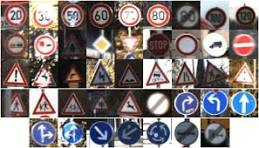
\includegraphics[scale=1.5]{figure2.jpg}
\caption{Some images used in the German Traffic Signs Recognition Benchmark}
\end{figure}


\chapter{Installation of the tools}
\tab For the installation of the alpha-beta-CROWN, we have used the step by step "Instructions for running the VNN-COMP benchmarks"\cite{alpha-beta-instructions} published by the tool developers which contains everything required for a successful installation. Firstly we cloned the git project recursively which also cloned auto\_LiRPA\cite{auto_lirpa_repo} to also support a wide range of neural network architectures.

After having the project locally, we installed Miniconda\cite{miniconda} to be able to have a fresh environment in which we can install the dependencies and run the tool on our benchmark. Here we ran into our first problem, which appeared to be that when trying to create the environment with Miniconda\cite{miniconda}, the yaml extension file defined to specify the dependencies when creating the environment, was containing a redirection to another yaml extension file. The specified redirection did not work and we had to move the dependencies from the redirected yaml extension file to the main yaml extension file.

Once we successfully used the correct yaml file for environment configuration, we ran into our second problem, which was the fact that not all of the dependencies used for alpha-beta-CROWN are available for Windows, therefore we had to change the operating system to a Linux based one and try again.

Finally, when we retried all of the steps with the adaptations written above, the installation was successful and the environment was ready for running benchmarks.

A problem that we encountered on the journey after the installation, was that each time we started the environment, we had to redefine the system variable VNNCOMP\_PYTHON\_PATH which contains the path to python, otherwise the run was not possible to start.
\chapter{Run of one tool for the benchmark}
\tab When it comes on running the benchmark, we have reached the conclusion that the first benchmark, tllverifybench\cite{tll_verify_bench}, was too simple and flawless to be able to extend the project after a simple run that reproduced the exact output from the competition. Therefore we chose to change it to Traffic Signs Recognition\cite{traffic_signs_recognition} so we can try to solve some of the problems that the competition run had.

After the first run we observed that due to a timeout after an instance that timed out, we could not reproduce the exact output due to the process stopping at that point, generating the report only to that specific instance (see

results\_traffic\_signs\_recognition\_default\_time.csv\cite{traffic_signs_recognition_first_solution}). After increasing the timeout in run\_all\_categories.sh file found in the alpha-beta-CROWN project, we were able to reproduce the output, but the instance that crashed the process still timed out, this time after 1000.0 seconds (the given value (see

results\_traffic\_signs\_recognition\_increased\_time\_to\_1000.csv\cite{traffic_signs_recognition_second_solution}).

\vspace{8pt}
\begin{tabular}{ |p{3cm}|p{3cm}|  }
 \hline
 \multicolumn{2}{|c|}{Traffic Signs Recognition benchmark run with alpha-beta-CROWN} \\
 \hline
 Falsified& 39\\
 \hline
 Penalty   & 3\\
 \hline
\end{tabular}
\vspace{10pt}

The falsified responses comes from the fact that the output for most of the instances seem to be satisfiable, when in fact there is still generated an counter-example for 39 of them which turn to be a false positive. The penalty comes from 3 instances that have the result different than "sat" or "unsat", 2 of them have the result "no\_result\_in\_file". After having a look in the logs, it appears that the branch-and-bound (BaB) round 69 stops (kills) the process in both instances therefore there is no output file from which to get the result. No successful method in changing the BaB and timeout configurations was found yet after some failed attempts.

The remaining instance that fails with the "run\_instance\_timeout" seems to not be fixed after increasing the timeout from 480 seconds to 1000, further timeout increase will be made to test if any real timeout value can fix the problem.
\begin{thebibliography}{1}
\bibitem{alpha-beta-instructions} Alpha-beta-CROWN instructions for running the VNN-COMP benchmarks, "https://github.com/Verified-Intelligence/alpha-beta-CROWN/blob/main/complete\_verifier/docs/vnn\_comp.md"
\bibitem{auto_lirpa_repo} Auto-LiRPA repository, "https://github.com/Verified-Intelligence/auto\_LiRPA"
\bibitem{miniconda} Miniconda, "https://docs.conda.io/projects/miniconda/en/latest/"
\bibitem{tll_verify_bench} TLLVerifyBench repository, "https://github.com/jferlez/TLLVerifyBench"
\bibitem{traffic_signs_recognition} Traffic Signs Recognition Repository, "https://github.com/ChristopherBrix/vnncomp2023\_benchmarks/tree/main/benchmarks/traffic\_signs\_recognition"
\bibitem{traffic_signs_recognition_first_solution} results\_traffic\_signs\_recognition\_default\_time.csv
"https://github.com/RafaelBan/VFProject/blob/main/results\_traffic\_signs\_recognition\_default\_time.csv"
\bibitem{traffic_signs_recognition_second_solution} results\_traffic\_signs\_recognition\_increased\_time\_to\_1000.csv
"https://github.com/RafaelBan/VFProject/blob/main/results\_traffic\_signs\_recognition\_increased\_time\_to\_1000.csv"
\bibitem{traffic_signs_paper}
Architecturing Binarized Neural Networks for Traffic Sign Recognition
"https://arxiv.org/abs/2303.15005"
\end{thebibliography}
\end{document} 